Exercise 1.4 contains data on three variables for the world's 10 largest companies as of
April 2005. For the sales ($x_{1}$) and profits ($x_{2}$) data:
\begin{enumerate}[label= (\alph*)]
    \item Construct Q-Q plots. Do these data appear to be normally distributed? Explain.
    \begin{figure}[H]
        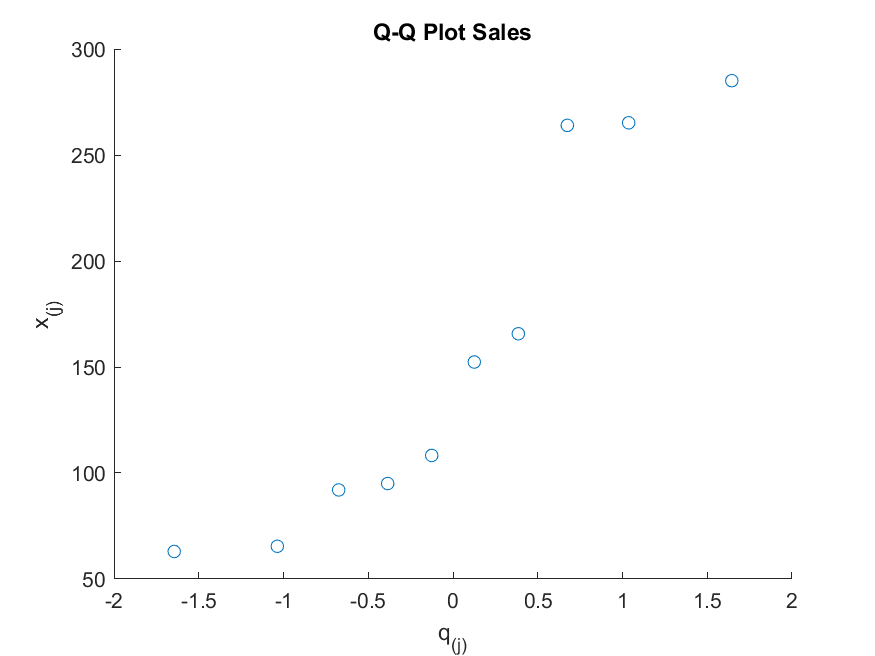
\includegraphics[scale=0.8]{./matlab/chapter-4/sol4.24a_sales.png}
    \end{figure}
    \begin{figure}[H]
        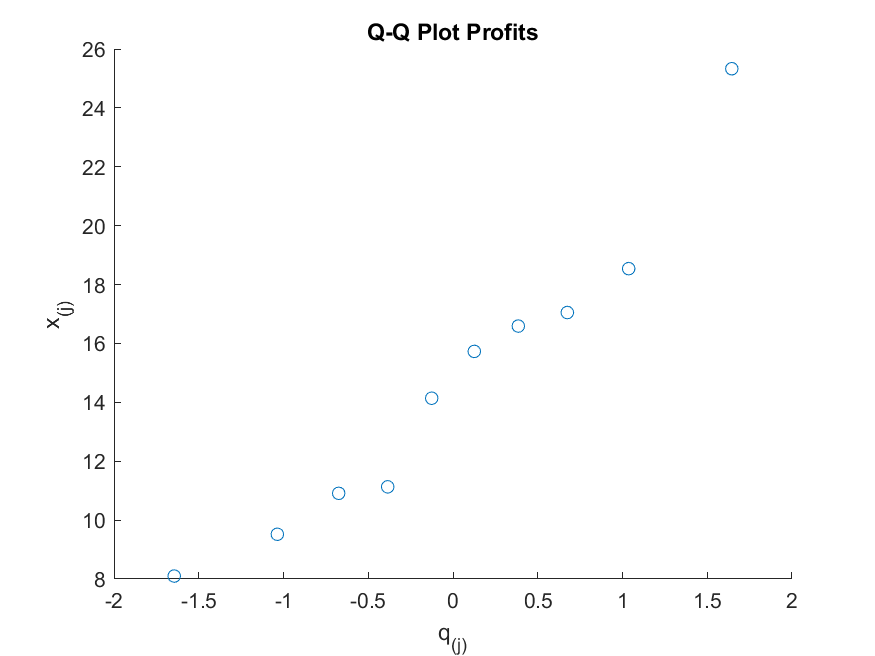
\includegraphics[scale=0.8]{./matlab/chapter-4/sol4.24a_profits.png}
    \end{figure}
    The Q-Q plot for sales does not really look linear, but the plot for profits does.
    \item Carry out a test of normality based on the correlation coefficient $r_{Q}$. [See (4--31).]
    Set the significance level at $\alpha = .10$. Do the results of these tests corroborate the results in Part a?
    \[
        r_{Q, \text{sales}}
        \frac{\mathlarger{\sum_{j=1}^{n}}{\left(x_{(j)} - \bar{x}\right)\left(q_{(j)} - \bar{q}\right)}}{\sqrt{\mathlarger{\sum_{j=1}^{n}}{\left(x_{(j)} - \bar{x}\right)}^{2}}\sqrt{\mathlarger{\sum_{j=1}^{n}}{\left(q_{(j)} - \bar{q}\right)}^{2}}}
        =
        \frac{721.0797}{\sqrt{67288}\sqrt{8.7979}}
        =
        0.9372
    \]
    \[
        r_{Q, \text{profits}}
        \frac{\mathlarger{\sum_{j=1}^{n}}{\left(x_{(j)} - \bar{x}\right)\left(q_{(j)} - \bar{q}\right)}}{\sqrt{\mathlarger{\sum_{j=1}^{n}}{\left(x_{(j)} - \bar{x}\right)}^{2}}\sqrt{\mathlarger{\sum_{j=1}^{n}}{\left(q_{(j)} - \bar{q}\right)}^{2}}}
        =
        \frac{44.1345}{\sqrt{235.7128}\sqrt{8.7979}}
        =
        0.9692
    \]
    In the book, from Table 4.2, with a sample size $n = 10$, the significance level is 0.9351.
    Performing the simulation using MATLAB, the significance level for 10M simulations was 0.9345.
    For sales, $r_{Q} = 0.9372$, which is slightly larger than the 0.1 significance level values of 0.9351 and 0.9345, so the sales column would be considered normally disributed.
    For profits, $r_{Q} = 0.9692$, which is larger than the 0.1 significance level values of 0.9351 and 0.9345, so the profits column would also be considered normally disributed.
\end{enumerate}